\documentclass[aps,pra,reprint,superscriptaddress,nofootinbib]{revtex4-2}
\usepackage{amsmath,amssymb,bm,graphicx}
\usepackage[colorlinks=true,linkcolor=blue,citecolor=blue,urlcolor=blue]{hyperref}
\newcommand{\spec}{\operatorname{spec}}
\newcommand{\Tr}{\operatorname{Tr}}
\newcommand{\ii}{\mathrm{i}}
\begin{document}
\title{Observable-dependent relaxation near a fermionic Liouvillian exceptional point}
\hypersetup{pdftitle={Observable-dependent relaxation near a fermionic Liouvillian exceptional point}}
\begin{abstract}
Which part of an exceptional-point spectrum governs a physical relaxation signal? For the uniformly pumped, post-selected quadratic-fermion model of Xu and Yi, we distinguish the unrestricted spectral gap, the parity-even gap, and the decay rates of specific observables. Total particle number and a difference of two mode occupations probe different collective-spin blocks. We derive exact reduced dynamics for both signals from the same positive, parity-even initial state. A fixed-order semiclassical expansion predicts the large-system ratio $1:2:\sqrt{2(d+1)}$ between the unrestricted gap, occupation-imbalance decay, and particle-number decay for $d$-fermion pumping. Direct propagation verifies the separation and shows how unequal readout weights mix a slower tail into the particle-number signal. The trace-nonincreasing domain and survival probability are included explicitly: a finite conditional decay rate can coexist with a rapidly vanishing post-selection yield. The results give a model-specific quantitative realization of known observable-sector selection, with exact identities separated from semiclassical assumptions.
\end{abstract}
\maketitle

\emph{Introduction.---}
The spectrum of a Liouvillian exceptional point describes possible decay modes, but a measurement samples only the modes allowed by the initial state and the observable. Symmetry selection can therefore produce different relaxation rates for different observables, as demonstrated by van Caspel and Gritsev~\cite{vanCaspel}. Fermions impose a further restriction: a physical density matrix is even under fermion parity, whereas the formally slowest mode of the full operator space may be odd. In conditional dynamics, normalization introduces an additional distinction between relaxation toward a limiting state and the probability of retaining a trajectory.

These distinctions can be resolved explicitly in the high-order exceptional-point model of Xu and Yi~\cite{XuYi}. Uniform $d$-fermion creation unfolds its size-$(n+1)$ Jordan block with the established exponent $1/(d+1)$. Here we ask which of the resulting spectral separations appear in one-time measurements of total occupation and occupation imbalance. Both signals can be prepared in the same full-rank, even state, yet they probe different spin representations and relax at different rates. We derive their exact reduced evolution, test it against the complete fermionic superoperator, and calculate the effect of unequal readout weights. A large-spin expansion supplies quantitative rate ratios and their finite-size approach. Neither observable-sector selection itself nor the fractional unfolding exponent is claimed as a new principle.

\emph{Conditional model and observables.---}
For $n\ge2$ fermion modes, $H=\sum_{ij}h_{ij}c_i^\dagger c_j$ with $h=h^\dagger$, consider the unnormalized evolution $\dot{\widetilde\rho}=\mathcal L\widetilde\rho$,
\begin{align}
\mathcal L\rho={}&-\ii[H,\rho]+\gamma\sum_j c_j\rho c_j^\dagger-n\gamma\rho
 +z\gamma\sum_{|I|=d}c_I^\dagger\rho c_I .
\label{eq:model}
\end{align}
Here $\gamma>0$, $1\le d\le n$, and $c_I^\dagger=c_{i_1}^\dagger\cdots c_{i_d}^\dagger$ for $i_1<\cdots<i_d$. Every $d$-mode subset has the same coefficient. The last term is recycling only, as in Ref.~\cite{XuYi}; adding pump anticommutators would change the model. Uniform sums are invariant under a single-particle basis rotation, since the creation channels transform by its unitary $d$th exterior power. We henceforth label the energy eigenmodes of $h$ and write $n_j=c_j^\dagger c_j$, $\hat N=\sum_j n_j$.

The map is completely positive for $z\ge0$. Its trace satisfies
\begin{equation}
\mathcal L^\dagger\mathbb1=\gamma\left[-(n-\hat N)+z\binom{n-\hat N}{d}\right].
\end{equation}
It is trace nonincreasing precisely when
\begin{equation}
0\le z\le \frac{n}{\binom nd}.
\label{eq:physical}
\end{equation}
The omitted jump can then have squared amplitude $\gamma[n-\hat N-z\binom{n-\hat N}{d}]\ge0$, completing a trace-preserving measurement instrument. The conditional state and survival weight are
\begin{equation}
\rho(t)=\frac{\widetilde\rho(t)}{P_{\rm surv}(t)},\qquad
P_{\rm surv}(t)=\Tr\widetilde\rho(t).
\label{eq:conditional}
\end{equation}
We take $z>0$ within Eq.~\eqref{eq:physical}; the defective $z=0$ endpoint is separate.

Choose the two even observables $\hat N/n$ and $D=n_1-n_2$, and the initial state
\begin{equation}
\rho_0=\rho_p(1+\epsilon D),\qquad
\rho_p=p^{\hat N}(1-p)^{n-\hat N},
\label{eq:initial}
\end{equation}
with $0<p<1$ and $0<|\epsilon|<1$. Since $D\in\{-1,0,1\}$ and $\Tr(\rho_pD)=0$, this state is normalized and strictly positive. It commutes with fermion parity $\Pi=(-1)^{\hat N}$, although it has support on both even and odd particle numbers. These are distinct notions of parity. Initially, $\langle\hat N\rangle_0=np$ and $\langle D\rangle_0=2\epsilon p(1-p)$.

\emph{Two exact observable channels.---}
Define the aggregate-population matrix $B_{M,d}(z)$, of dimension $M+1$, by
\begin{equation}
B_{k-1,k}=k,\qquad B_{k+d,k}=z\binom{M-k}{d},
\label{eq:B}
\end{equation}
with all other entries zero. Let $F_{M,k}=\binom Mk p^k(1-p)^{M-k}$ and $R_M(t)=e^{\gamma t B_{M,d}(z)}F_M$. For the state~\eqref{eq:initial}, the complete conditional signals reduce exactly to
\begin{align}
\frac{\langle\hat N\rangle_t}{n}
 &=\frac{\sum_{k=0}^n(k/n)R_{n,k}(t)}{\sum_{k=0}^nR_{n,k}(t)},\nonumber\\
\langle D\rangle_t
 &=2\epsilon p(1-p)\frac{\sum_{k=0}^{n-2}R_{n-2,k}(t)}{\sum_{k=0}^nR_{n,k}(t)},\label{eq:signals}\\
P_{\rm surv}(t)&=e^{-n\gamma t}\sum_{k=0}^nR_{n,k}(t).\nonumber
\end{align}
Thus the entire particle-number and survival curves are independent of $\epsilon$, while the imbalance is proportional to it. No odd density matrix or odd measurement is used.

The selection rule follows directly on the diagonal Boolean space. Write $P_k$ for the unnormalized $k$-particle projector, and $J_\pm=\sum_j\sigma_j^\pm$ for adding or removing occupied modes. The recycling matrix is $G_{n,d}=J_-+zJ_+^d/d!$. The $P_k$ span spin $n/2$. In contrast, with $m=n-2$ and $Q_k=DP_{k+1}$,
\begin{equation}
J_-Q_k=(m-k+1)Q_{k-1},\qquad
J_+Q_k=(k+1)Q_{k+1}.
\label{eq:selection}
\end{equation}
The first two Boolean spins form a singlet, leaving one spin-$m/2$ copy. Moreover, $\Tr Q_k=\Tr(\hat NQ_k)=0$ and $\Tr(DQ_k)=2\binom mk$. These identities prove Eq.~\eqref{eq:signals}. They also show why occupation imbalance is absent from the normalization denominator. Off-diagonal energy-basis coherences do not feed these diagonal channels. Details and more general initial-state projections are given in the accompanying Supplemental Material.

\begin{figure*}[t]
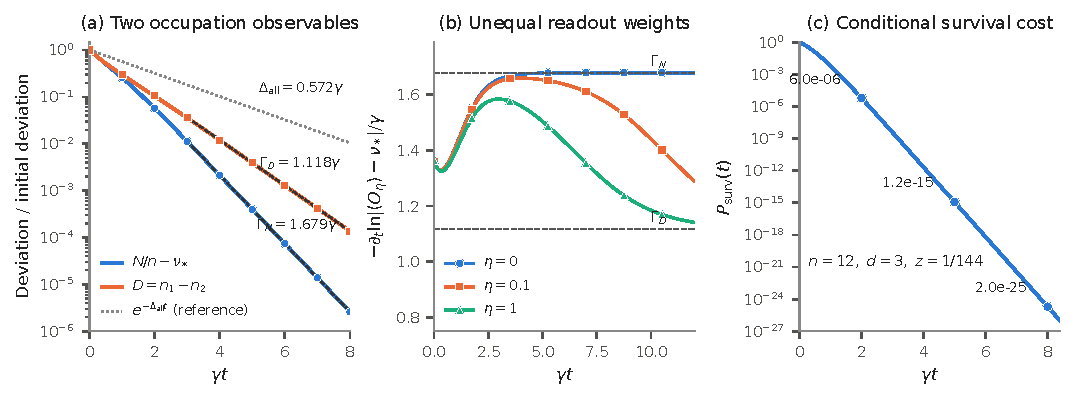
\includegraphics[width=\textwidth]{../figs/observable_dynamics.pdf}
\caption{Conditional dynamics from the same full-rank state, Eq.~\eqref{eq:initial}, with $p=0.75$, $\epsilon=0.6$, $n=12$, $d=3$, and $z=1/144$. (a) Particle-number and occupation-imbalance deviations, each divided by its initial value. Dashed curves use spectral amplitudes and rates, without fitting. The dotted unrestricted-gap reference describes neither signal. (b) Effective logarithmic decay rate for $O_\eta=\hat N/n+\eta D/n$. Unequal weights mix the slower imbalance into the readout. Horizontal dashed lines mark $\Gamma_N$ and $\Gamma_D$. (c) Survival probability for the same evolution. The long-time tails occur at very low post-selection yield; the plots establish conditional exponents, not an efficient measurement protocol.}
\label{fig:dynamics}
\end{figure*}

\emph{Visible rates and the parity restriction.---}
Let $q=z^{1/(d+1)}$ and $\kappa_{M,d}$ be the Perron root of $B_{M,d}(1)$, setting $\kappa_{M,d}=0$ for $M<d$. A diagonal similarity with entries $q^k$ gives $B_{M,d}(z)\sim qB_{M,d}(1)$. Define the maximal-block real-part separation
\begin{equation}
\delta_{n,d}=\kappa_{n,d}-\max_{\nu\in\spec B_{n,d}(1),\,\nu\ne\kappa_{n,d}}\Re\nu.
\label{eq:delta}
\end{equation}
The leading eigenvalue is $\lambda_*=-n\gamma+\gamma q\kappa_{n,d}$. For $n-2\ge d$, positivity of the initial projection in Eq.~\eqref{eq:signals} guarantees a nonzero imbalance Perron amplitude. Consequently,
\begin{align}
\langle D\rangle_t&\sim A_D e^{-\Gamma_D t},&
\Gamma_D&=\gamma q(\kappa_{n,d}-\kappa_{n-2,d}),\nonumber\\
\langle\hat N\rangle_t/n-\nu_*&\sim A_N e^{-\Gamma_Nt},&
\Gamma_N&=\gamma q\delta_{n,d},
\label{eq:rates}
\end{align}
where $\nu_*$ is the limiting filling. The second line assumes a real subleading root with nonzero normalized observable overlap, as verified for the examples below. In general one takes the largest real part among the roots with nonzero overlap after subtracting $\nu_*$ times the trace. Complex roots give oscillations, and Jordan roots can give polynomial prefactors. A positive initial state alone does not guarantee a particle-number transient: a stationary conditional state has none. When $n-2<d$, the imbalance block is nilpotent and the positive initial state~\eqref{eq:initial} instead gives $t^{n-2}e^{-\gamma q\kappa_{n,d}t}$ at long times.

To compare these rates with the full spectral gaps, label an operator by disjoint sets $A,B$ occupied only on its ket or bra, respectively. On the $m=n-|A|-|B|$ remaining common modes, a diagonal sign gauge turns the recycling into $G_{m,d}$. The Hamiltonian adds only $-\ii(E_A-E_B)$, and the spin decomposition of $G_{m,d}$ supplies blocks $B_{m-2j,d}$ with multiplicity $\binom mj-\binom m{j-1}$. This gives the complete spectrum without diagonalizing a $4^n$ matrix. Quadratic-fermion Jordan methods provide context~\cite{Prosen}; the $d>1$ pump here is not quadratic in fermionic superoperators.

An operator is parity even precisely when $|A|+|B|$ is even. Positivity and principal-submatrix embedding of the Boolean matrices imply monotonic $\kappa_{m,d}$. The exact gaps are therefore
\begin{align}
\Delta_{\rm all}&=\gamma q\min\{\delta_{n,d},\kappa_{n,d}-\kappa_{n-1,d}\},\nonumber\\
\Delta_{\rm even}&=\gamma q\min\{\delta_{n,d},\kappa_{n,d}-\kappa_{n-2,d}\}.
\label{eq:gaps}
\end{align}
Neither minimum can generally be omitted. For example, $n=d=4$, $z=1$ is physical, but the maximal block's complex roots give $\Delta_{\rm even}=\gamma24^{1/5}[1-\cos(2\pi/5)]<\Gamma_D$. Parity-even one-time measurements exclude odd intermediate modes. This restriction does not exclude odd sectors from fermionic two-time Green functions, whose insertions and conditional measurement protocol must be specified separately.

\emph{Dynamics and readout mixing.---}
Figure~\ref{fig:dynamics} compares the two signals from one state. For $n=12$, $d=3$, and $z=1/144$, the exact small-matrix spectra give
\begin{equation}
(\Delta_{\rm all},\Gamma_D,\Gamma_N)/\gamma
=(0.571963,\,1.117616,\,1.678630).
\label{eq:numbers}
\end{equation}
Here $\Delta_{\rm even}=\Gamma_D$, but total particle number relaxes faster. Propagation gives the same rates and spectral amplitudes for $(n,d)=(8,2),(12,3),(16,4)$. The reduced population dynamics retain the occupations of two marked modes and the remaining occupation count; they agree with direct full-superoperator evolution for three small systems to below $2\times10^{-15}$. Integer intertwining identities check Eq.~\eqref{eq:selection} for $2\le n\le7$ and all $d\le n$.

A detector with unequal weights on modes 1 and 2 measures
\begin{equation}
O_\eta=\frac{\hat N}{n}+\eta\frac{D}{n}.
\end{equation}
Whenever $\Gamma_D<\Gamma_N$ and both amplitudes are nonzero,
\begin{equation}
\langle O_\eta\rangle_t-\nu_*\simeq
 A_N e^{-\Gamma_Nt}+\frac{\eta A_D}{n}e^{-\Gamma_Dt}.
\label{eq:readout}
\end{equation}
Every fixed $\eta\ne0$ then selects the slower asymptotic exponent, whereas $\eta=0$ retains $\Gamma_N$. Equating the magnitudes gives
\begin{equation}
t_\times\simeq\frac{\ln[n|A_N|/(|\eta A_D|)]}{\Gamma_N-\Gamma_D}.
\label{eq:cross}
\end{equation}
This is the usual competition of two exponentials, now with explicit sector rates and amplitudes. For Fig.~\ref{fig:dynamics}, $A_N=0.726392$ and $A_D=0.235641$ follow from left and right eigenvector projections; $\eta=0.1$ gives $\gamma t_\times\simeq10.54$. Already at $\gamma t=5$, however, $P_{\rm surv}=1.18\times10^{-15}$, falling to $2.02\times10^{-25}$ at $\gamma t=8$. The asymptotic readout sensitivity is consequently a statement about conditioned signals, not a claim of practical precision at those times.

\emph{Large-system hierarchy.---}
The collective-spin blocks also yield useful fixed-$d$ asymptotics. Define
\begin{align}
\alpha_d&=\frac{2d}{d+1},&\beta_d&=\frac{d-1}{d+1},&\Omega_d&=\sqrt{\frac{d+1}{2}},\nonumber\\
a_d&=\left[\frac{2^{-(d-1)}}{(d-1)!}\right]^{1/(d+1)},&&C_d=\frac{a_d}{\alpha_d}.
\end{align}
A nonunitary rotation of $J_-+zJ_+^d/d!$, followed by expansion about the polarized spin, gives a local oscillator $1-P^2-(d+1)X^2/2$. For fixed oscillator index $\ell$, the resulting formal edge ladder is
\begin{equation}
\mu_\ell=q\left\{C_dn^{\alpha_d}+a_d[1-(2\ell+1)\Omega_d]n^{\beta_d}
+O(n^{\beta_d-1})\right\}.
\label{eq:edge}
\end{equation}
Identifying the first two levels with the two largest positive radial roots predicts $\delta_{n,d}\sim2a_d\Omega_dn^{\beta_d}$ and $\kappa_{n,d}-\kappa_{n-r,d}\sim r a_dn^{\beta_d}$. Thus, for fixed $d>1$ and nonzero visible overlaps,
\begin{equation}
\Delta_{\rm all}:\Gamma_D:\Gamma_N
\ \longrightarrow\ 1:2:\sqrt{2(d+1)},\qquad
\Delta_{\rm even}\sim\Gamma_D.
\label{eq:hierarchy}
\end{equation}
For $d=1$, the spectrum is exactly $\mu_\ell=q(n-2\ell)$: $\Gamma_N=\Gamma_D=\Delta_{\rm even}=2\gamma q$, while $\Delta_{\rm all}=\gamma q$. Multiparticle pumping separates the two even-observable rates.

\begin{figure}[t]
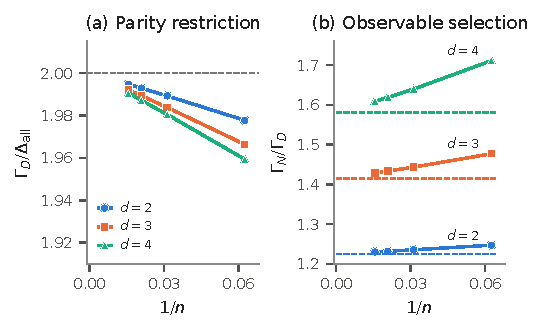
\includegraphics[width=\columnwidth]{../figs/rate_hierarchy.pdf}
\caption{Finite-size approach to the hierarchy, Eq.~\eqref{eq:hierarchy}. (a) Imbalance decay relative to the unrestricted gap tends to 2. For these sizes $\Gamma_D=\Delta_{\rm even}$. (b) Maximal-block spacing relative to imbalance decay tends to $\Omega_d=\sqrt{(d+1)/2}$; it is the particle-number rate when its overlap is nonzero. Symbols use $n=16,32,48,64$; dashed lines are parameter-free limits. Ratios are independent of $z>0$. Perron roots use log-space positive iteration, and internal gaps use independently repeated 50- and 70-digit spectra.}
\label{fig:hierarchy}
\end{figure}

Equation~\eqref{eq:edge} is a fixed-low-excitation expansion, not a norm bound over the full spin space. McMillen's double-band theorem~\cite{McMillen} excludes off-axis competitors on the local edge scale, but the radial-edge identification and a uniform spectral remainder are not proved here. Figure~\ref{fig:hierarchy}, together with spectral-edge data through $n=512$ in the Supplemental Material, supports the semiclassical prediction. For $d=2$, the leading coefficient $C_2=3/2^{7/3}$ is already implied by the quartic-potential result of Shapiro and Tater~\cite{ShapiroTater}. Structured-Jordan ring splitting is likewise established~\cite{MaEdelman,Graefe}. The Supplemental Material records the exact polynomial recurrence and explains the nonuniform use of the first-order truncation in Eq.~(54) of Ref.~\cite{XuYi} (arXiv v2 numbering), without changing that work's fractional exponent or its displayed $n=4$, $d=2,3,4$ tests.

Physical large-$n$ scaling requires reducing the weight per pump channel. With $z=\zeta n^{1-d}$ and fixed $0<\zeta<d!$, Eq.~\eqref{eq:physical} holds and the predicted rates approach finite values:
\begin{align}
\Gamma_D&\sim2\gamma a_d\zeta^{1/(d+1)},\quad
\Gamma_N\sim2\gamma a_d\Omega_d\zeta^{1/(d+1)},\nonumber\\
\frac{\lambda_*}{\gamma n}&=-1+C_d\zeta^{1/(d+1)}+O(n^{-1}).
\label{eq:physicalscaling}
\end{align}
For $d>1$, $C_d(d!)^{1/(d+1)}<1$, so survival still has an extensively negative long-time exponent. These are asymptotic exponents, not general bounds on transient relaxation times or experimental cost.

\emph{Scope.---}
The central exact result is the assignment of two accessible density observables to different finite spin blocks, including the normalization denominator. It makes the parity restriction, observable selection, and readout mixing separately testable in one conditional model. The large-$n$ hierarchy adds a quantitative semiclassical prediction rather than a new general selection principle. Uniform channels and number-conserving quadratic $H$ are essential; nonuniform reservoirs, pairing, and additional dissipator terms require a new analysis. All calculations and source checks are supplied, including the distinction between floating-point convergence diagnostics and rigorous bounds.

\bibliography{references}
\end{document}
